% !TeX spellcheck = it_IT
\documentclass[10pt,a4paper]{article}

\usepackage[utf8]{inputenc}
\usepackage[T1]{fontenc}	
\usepackage[italian]{babel}
\usepackage{amsmath}
\usepackage{amsfonts}
\usepackage{amssymb}
\usepackage{graphicx}

\usepackage[left=2cm,right=2cm,top=2cm,bottom=2cm]{geometry}
\geometry{a4paper}

\usepackage{booktabs} % for much better looking tables
\usepackage{verbatim}
\usepackage{subfig} % make it possible to include more than one captioned figure/table in a single 

\usepackage{fancyhdr} % This should be set AFTER setting up the page geometry
\pagestyle{fancy} % options: empty , plain , fancy
\renewcommand{\headrulewidth}{0pt} % customise the layout...
\lhead{}\chead{}\rhead{}
\lfoot{}\cfoot{\thepage}\rfoot{}

%%% SECTION TITLE APPEARANCE
\usepackage{sectsty}
%\allsectionsfont{\sffamily\mdseries\upshape} % (See the fntguide.pdf for font help)
% (This matches ConTeXt defaults)

% pacchetti che mi fanno schifo ma uso lo stesso (Bob è scemo, ma anche Ale...)
\usepackage[cdot, thickqspace, squaren]{SIunits}
% il miglior pacchetto che potessi desiderare
\usepackage{float}
% macro che mi piacciono
\def\code#1{\texttt{#1}}


\title{Esercitazione 6: Amplificatore operazionale, Circuiti lineari}

\author{Gruppo BE \\ Alessandro Candido, Roberto Ribatti}
\date{\today}
\begin{document}
\maketitle

\section{Scopo e strumentazione}
Misurare le caratteristiche di amplificatori invertenti e non invertenti realizzati con un op-amp TL081, da alimentare tra +15 V e -15V. Misurare la risposta di un circuito derivatore e di un circuito integratore realizzati col suddetto op-amp.
La strumentazione usata è quella presente sul banco di lavoro, più il suddetto transistor.

\section{Amplificatore invertente}
Si è realizzato l'amplificatore invertente mostrato in \figurename{\ref{circuito_amp_inv}} e si sono scelte le resistenze $R_1$ e $R_2$ rispettivamente di $\unit{10}{k\ohm}$ e $\unit{100}{k\ohm}$ in modo da avere un impedenza di ingresso pari a $\sim \unit{10}{k\ohm}$, maggiore di $\unit{1}{k\ohm}$ e un guadagno pari a $R_2/R_1 \sim 10$, come richiesto. Di seguito i valori misurati delle resistenze:
\begin{figure}[H]
\begin{minipage}{0.49\textwidth}
	\centering
	\begin{tabular}{cc}
		$R_1 = \unit{9.89 \pm 0.09}{k\ohm}$  \\ $R_2 = \unit{98.5 \pm 0.9}{k\ohm}$
	\end{tabular}
\end{minipage}
\begin{minipage}{0.49\textwidth}
	\centering
	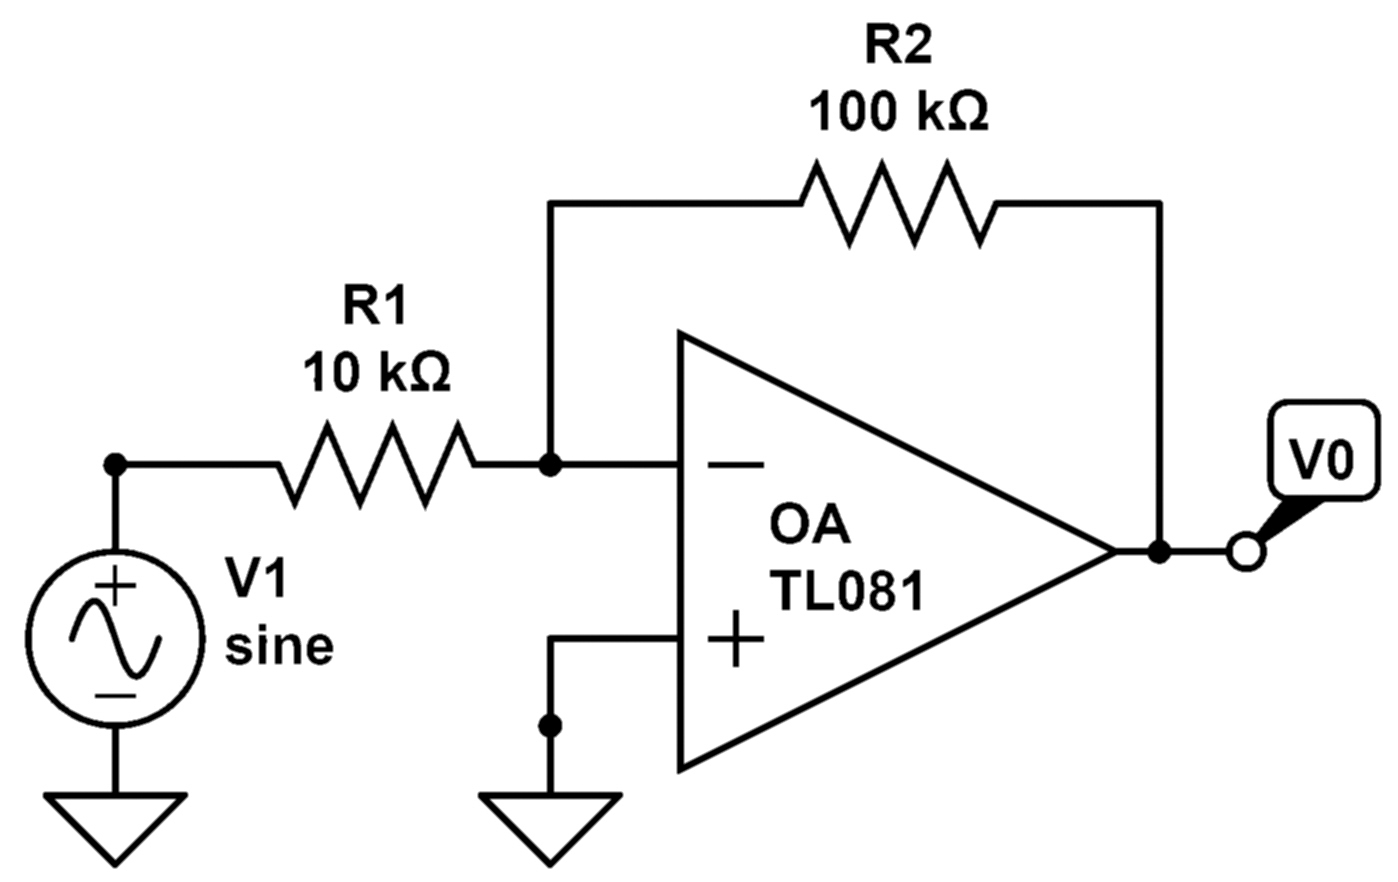
\includegraphics[width=0.7\textwidth]{../grafici/inv_amp_circuito.jpg}
	\caption{Circuito amplificatore invertente}
	\label{circuito_amp_inv}
\end{minipage}
\end{figure}

\subsection{Guadagno e linearità}
Si è misurata quindi la risposta del circuito ad un segnale sinusoidale di frequenza fissata $f = \unit{4.62 \pm 0.05}{k\hertz}$ al variare della tensione picco-picco del segnale in ingresso. I dati raccolti sono elencati in appendice in \tablename{\ref{tab:inv_amp_gain}}.

Dall'analisi del segnale all'oscilloscopio (vedi \figurename{\ref{fig:inv_amp}}) è visibile lo sfasamento di mezzo periodo tra i segnali, come atteso.

\begin{figure}[H]
	\centering
	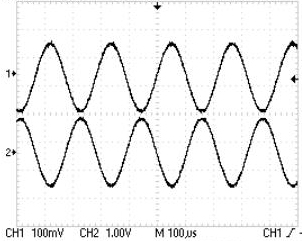
\includegraphics[width=0.45\textwidth]{../oscilloscopio/dinverting.jpg}
	\caption{Inversione di fase nell'amplificatore invertente}
	\label{fig:inv_amp}
\end{figure}

I dati mostrano un chiaro comportamento lineare fino a tensioni in ingresso di $\sim \unit{2.9}{\volt}$ cioè per tensioni di uscita vicine a $\unit{30}{\volt}$, in pratica il regime in cui l'op-amp è lineare. Si è fittato il guadagno nella zona lineare, i risultati e grafici del fit sono riportati di seguito:

\begin{table}[H]
	\centering
	\begin{tabular}{ccc}
		$|A_v| = 9.72 \pm 0.08$  & intercetta: $\unit{0.04 \pm 0.03}{\volt}$ & $\chi^2/ndof= 8.5 / 23$
	\end{tabular}
\end{table}
Il guadagno misurato è compatibile con quello atteso dalla teoria ($|A_v|^{exp} = 9.96 \pm 0.13$) a meno di $2\sigma$, il valore del $\chi^2$ risulta tuttavia essere molto basso, ciò è dovuto evidentemente ad una sovrastima degli errori statistici, dovuto alla sensibilità dell'oscilloscopio.
\begin{figure}[H]
	\centering
	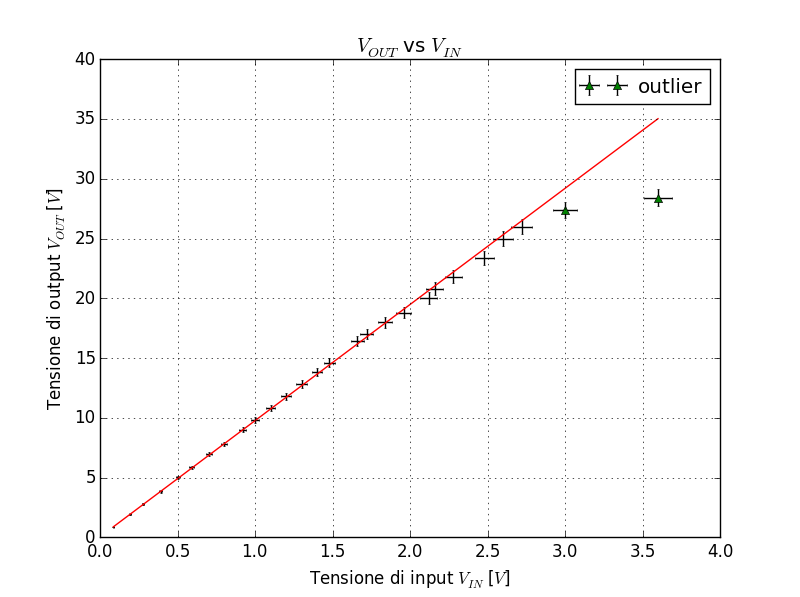
\includegraphics[width=0.85\textwidth]{../grafici/fit_inv_amp_gain.pdf}
	\caption{Guadagno amplificatore invertente}
	\label{fig:inv_amp_gain}
\end{figure}
 
\subsection{Impedenza d'ingresso}
Si è proceduto alla misura della impedenza di ingresso, per farlo si è posta una resistenza $R^* = \unit{9.96 \pm 0.09}{k\ohm}$ in serie all'ingresso del circuito e si è misurata la caduta di potenziale ai capi della stessa ottenendo:
\begin{table}[H]
	\centering
	\begin{tabular}{cc}
		$V_1 = \unit{2.88 \pm 0.10}{\volt}$  &  $V_2=\unit{1.44 \pm 0.05}{\volt}$
	\end{tabular}
\end{table}
L'impedenza di ingresso misurata è quindi $R_{IN}=\unit{10.0 \pm 1.0}{k\ohm}$, ampiamente compatibile con quella attesa pari a $R_1$.

\subsection{Risposta in frequenza}
Si è studiata quindi la risposta in frequenza del circuito, per una tensione picco-picco in ingresso pari a $V = \unit{496 \pm 12}{\milli\volt}$. I dati acquisiti sono riportati in appendice in \tablename{\ref{tab:inv_amp_f_domain}}.

Dal grafico in \figurename{\ref{palle}} è chiaro che il guadagno è costante fino ad un frequenza di $\sim \unit{200}{k\hertz}$, da questo punto in poi il guadagno sembra calare linearmente con un tasso di $\sim \unit{20}{\deci\bel /decade}$ per un primo tratto fino a $f \sim {600}{k\hertz}$, per frequenze superiori la pendenza sembra aumentare.

Si è provato a fittare questo comportamento (il grafico del fit è riportato in \figurename{\ref{rette}}), le pendenze fittate sono state $p_1 = \unit{-20.1 \pm 1.8}{\deci\bel/decade}$ per il primo tratto e $p_2 =\unit{-33.3 \pm 1.2}{\deci\bel/decade}$ per il secondo tratto.

\begin{figure}[H]
	\centering
	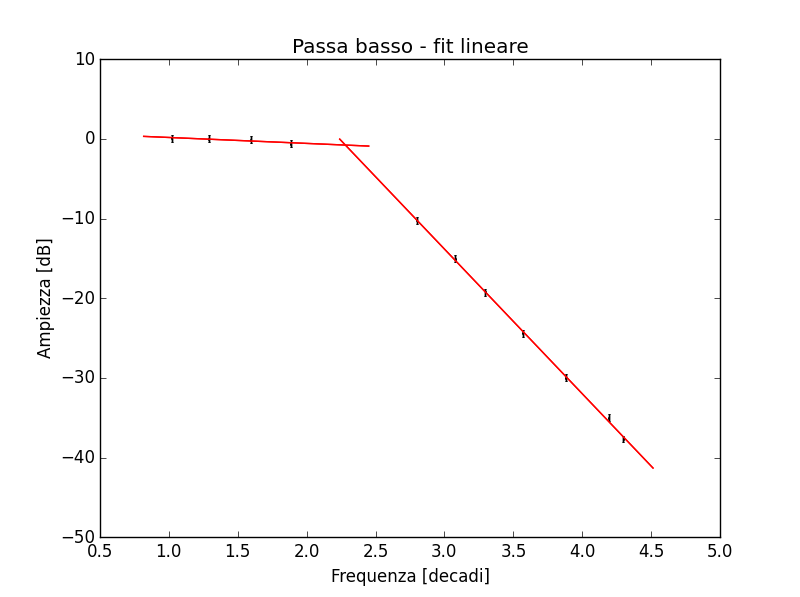
\includegraphics[width=0.7\textwidth]{../grafici/fit_rette.pdf}
	\caption{fit del guadagno per alte frequenze}
	\label{rette}
\end{figure}

Si è deciso quindi di fittare la risposta in frequenza dell'amplificatore invertente con il modello di un filtro passa basso escludendo i dati presi a frequenze sopra $\sim \unit{600}{k\hertz}$ che come visto prima non rispettano la legge di decrescita attesa.  Si riportano di seguito i risultati del fit e il grafico.

\begin{table}[H]
	\centering
	\begin{tabular}{ccc}
	$|A_v| = 10.15 \pm 0.13$	&	$f_0 = \unit{214 \pm 6}{k\hertz}$	&	$\chi^2/ndof = 23 / 20$\\
	\end{tabular}
\end{table}

\begin{figure}[H]
	\centering
	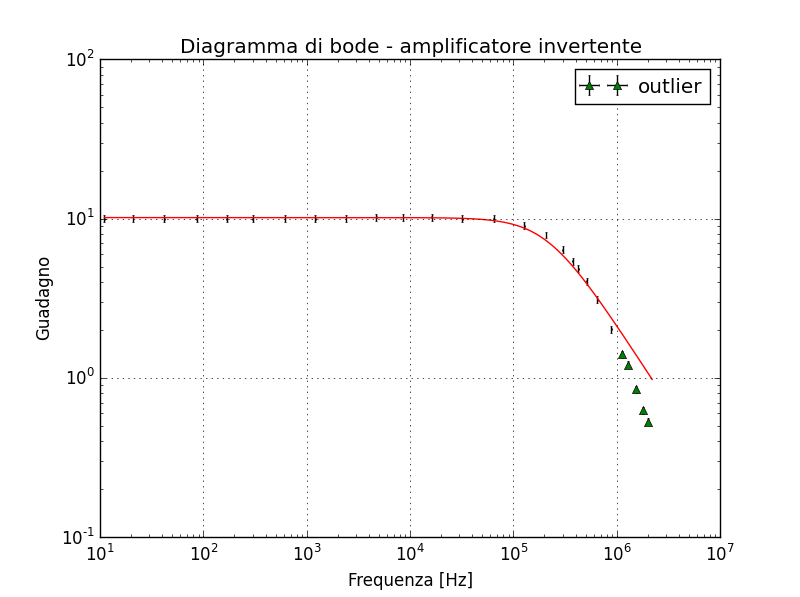
\includegraphics[width=0.8\textwidth]{../grafici/fit_inv_amp_f_domain.pdf}
	\caption{Grafico dei dati e del fit}
	\label{palle}
\end{figure}

Il guadagno di centro banda fittato è compatibile con quello atteso dalla teoria e con quello misurato al punto precedente.
L'andamento ad alte frequenze è probabilmente influenzato dallo slew rate che in questo range distorce significativamente il segnale.
\pagebreak
\subsection{Slew rate}
Si è misurato lo slew rate dell'op-amp inviando in ingresso un'onda quadra di frequenza $\unit{1000 \pm 10}{\hertz}$, ottenendo una discesa pari a  $\Delta V = \unit{9.44 \pm 0.24}{\volt}$ in un tempo $\Delta t = \unit{740 \pm 7}{\nano\second}$.

Lo slew rate misurato è quindi pari a $\unit{12.8 \pm 0.3}{\volt/\micro\second}$, compatibile con il valore tipico di $\unit{13}{\volt/\micro\second}$ riportato dal datasheet.

%gli errori sulle frequenze li abbiamo messi sempre all'1%?

\section{Amplificatore non invertente}

Si è montato l'amplificatore non invertente in \figurename{\ref{circuito_non_inv}} con $R_1 = \unit{218 \pm 3}{\ohm}$.

\begin{figure}[H]
	\centering
	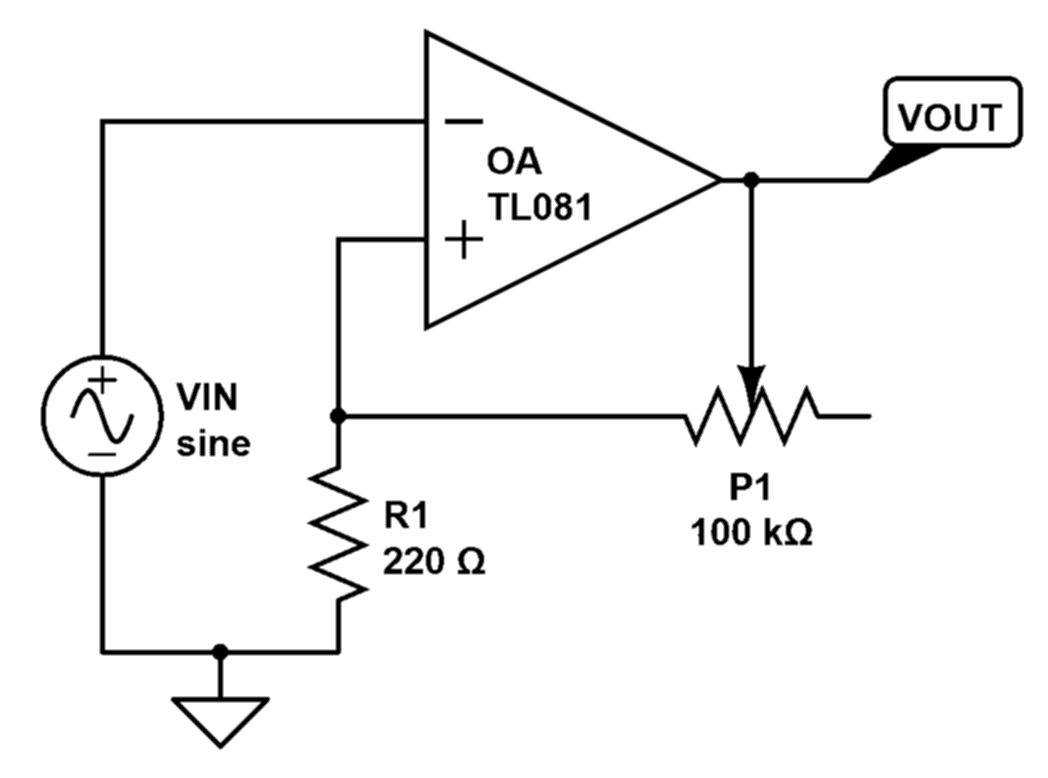
\includegraphics[width=0.4\textwidth]{../grafici/non_inv_amp_circuito.jpg}
	\caption{Circuito amplificatore non invertente}
	\label{circuito_non_inv}
\end{figure}

Si sono misurati al variare della posizione del potenziometro il guadagno (misurato a basse frequenze $f < \unit{100}{\hertz}$, dove sicuramente l'amplificatore è in regime lineare) e la frequenza di taglio superiore. I dati acquisiti sono riportati in appendice in \tablename{\ref{tab:gain_bandwidth}}. Per verificare che il prodotto banda-guadagno rimanesse costante si è fittato con una retta il guadagno (in decibel) in funzione del logaritmo della frequenza. I risultati e il grafico del fit sono riportati di seguito (a è il coefficiente angolare e b l'intercetta):

\begin{table}[H]
	\centering
	\begin{tabular}{ccc}
		$a = \unit{-20.49 \pm 0.18}{\deci\bel /decade}$  &  $b = \unit{128.8 \pm 0.8}{\deci\bel}$ & $\chi^2/ndof= 14.8 / 13$
	\end{tabular}
\end{table}

\begin{figure}[H]
	\centering
	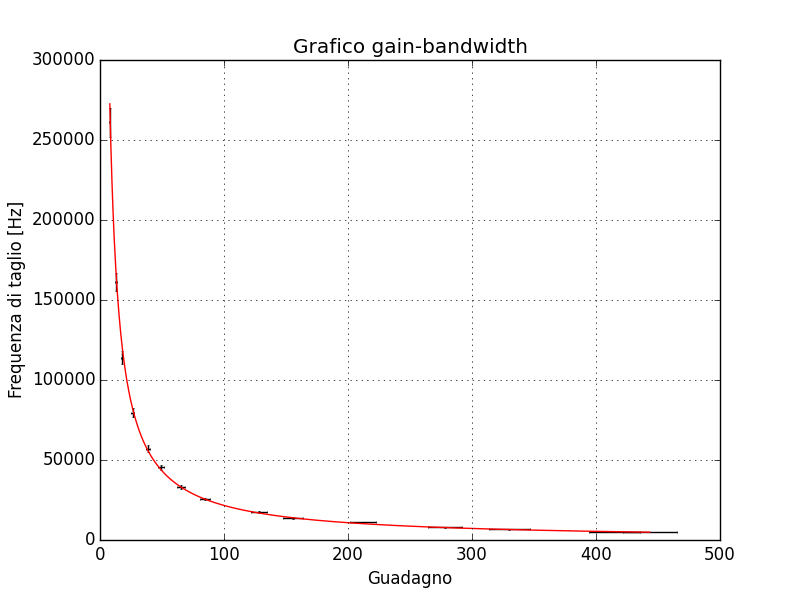
\includegraphics[width=0.8\textwidth]{../grafici/fit_gain_bandwidth.pdf}
	\caption{Grafico e fit guadagno-banda}
\end{figure}

Il prodotto banda guadagno, ovvero l'intersezione della retta fittata con l'asse a $\unit{0}{\deci\bel}$ varrà perciò\footnote{propagando l'errore tenendo conto della covarianza}: $Af_h=\unit{1.93\pm0.12}{\mega\hertz}$, che è da confrontarsi con il grafico presente nel datasheet riportato in \figurename{\ref{fig:open_loop_stocazzo}}.

\begin{figure}[H]
	\centering
	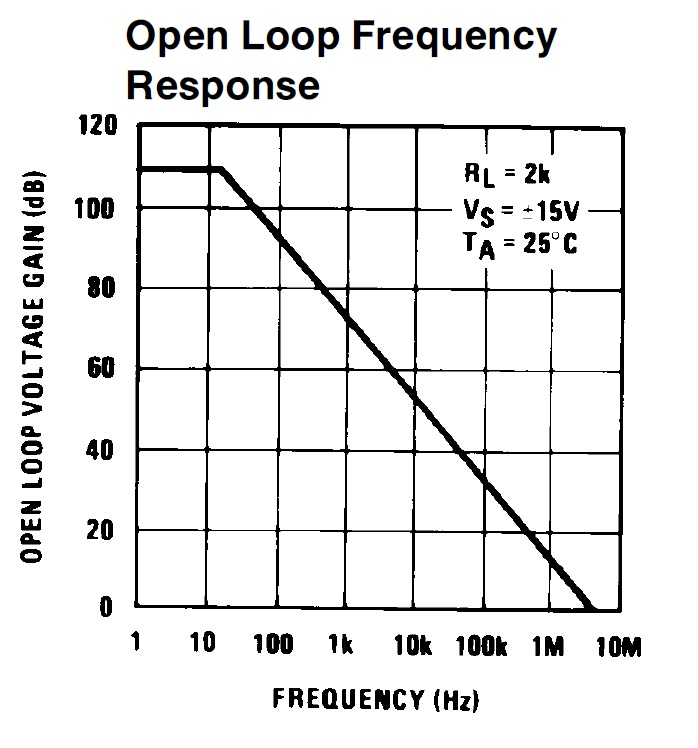
\includegraphics[width=0.45\textwidth]{../grafici/open_loop_frequency.jpg}
	\caption{Grafico guadagno-banda dal datasheet}
	\label{fig:open_loop_stocazzo}
\end{figure}

\section{Circuito integratore}

Si è montato il cirucito in \figurename{\ref{integratore}}. I valori dei componenti utilizzati sono:
\begin{figure}[H]
\begin{minipage}{0.49\textwidth}
\centering
\begin{tabular}{c}
$R_1 = \unit{984 \pm 9}{ohm}$	\\	$R_2 = \unit{9.95 \pm 0.09}{\kilo\ohm}$	\\	$C = \unit{45.4 \pm 1.8}{\nano\farad}$
\end{tabular}
\end{minipage}
\begin{minipage}{0.49\textwidth}
	\centering
	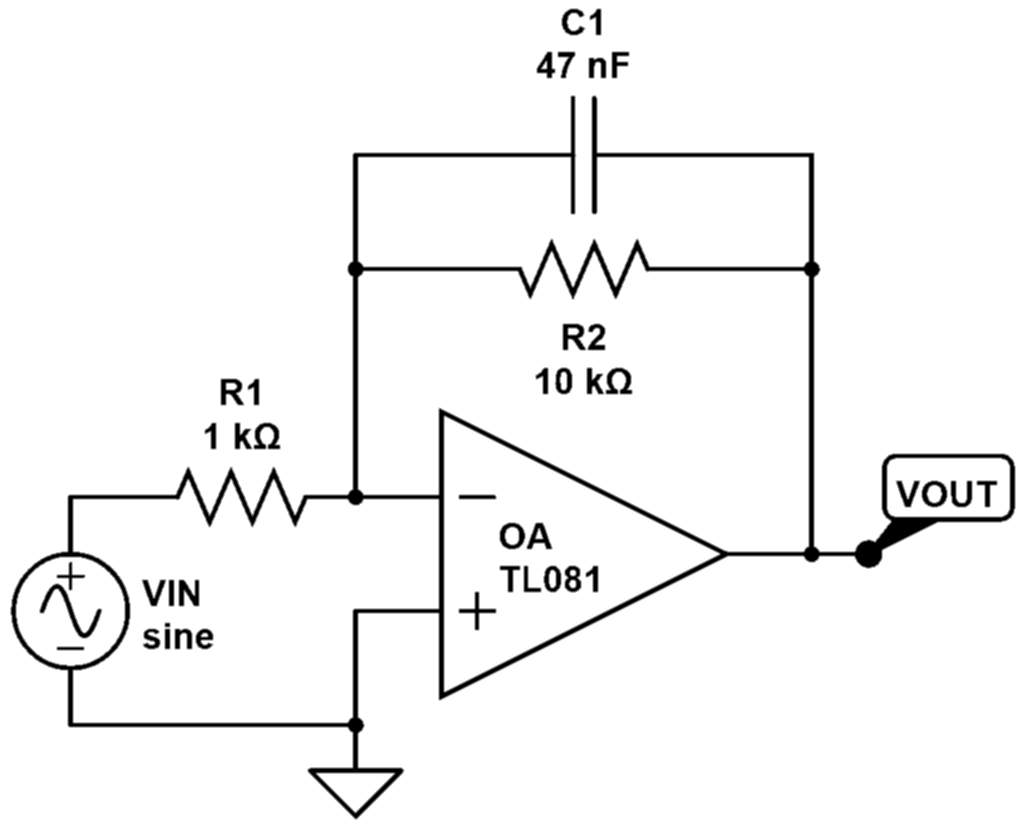
\includegraphics[width=0.8\textwidth]{../grafici/integratore_circuito.jpg}
	\caption{Circuito integratore}
	\label{integratore}
\end{minipage}
\end{figure}


\subsection{Risposta in frequenza}
Si è misurata la risposta del circuito a un ingresso sinusoidale a varie frequenze. Si riportano i dati relativi in appendice in \tablename{\ref{tab:lowpass}}, e i grafici di seguito in \figurename{\ref{fig:lowamp}} e \figurename{\ref{fig:lowph}}.
	\begin{figure}[H]
		\centering
		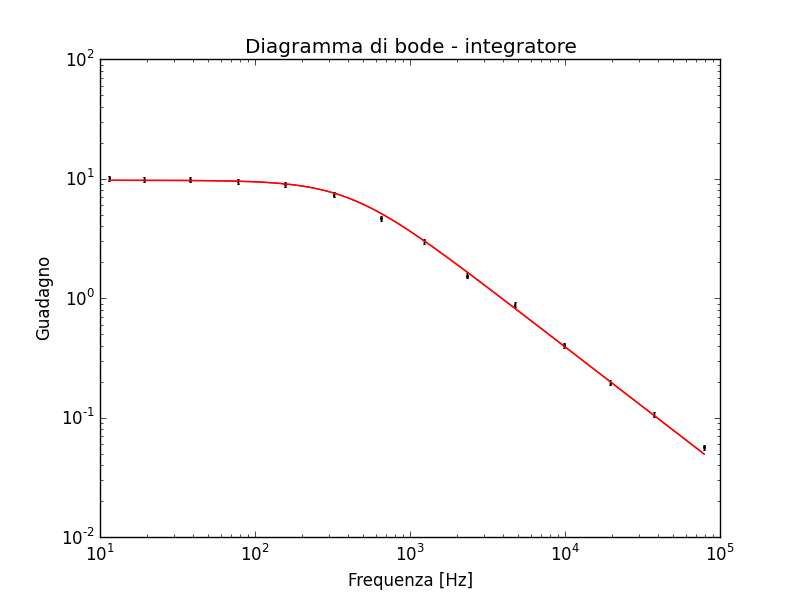
\includegraphics[width=0.8\textwidth]{../grafici/fit_module_low_pass.pdf}
		\caption{Guadagno integratore}
		\label{fig:lowamp}
	\end{figure}
	\begin{figure}[H]
		\centering
		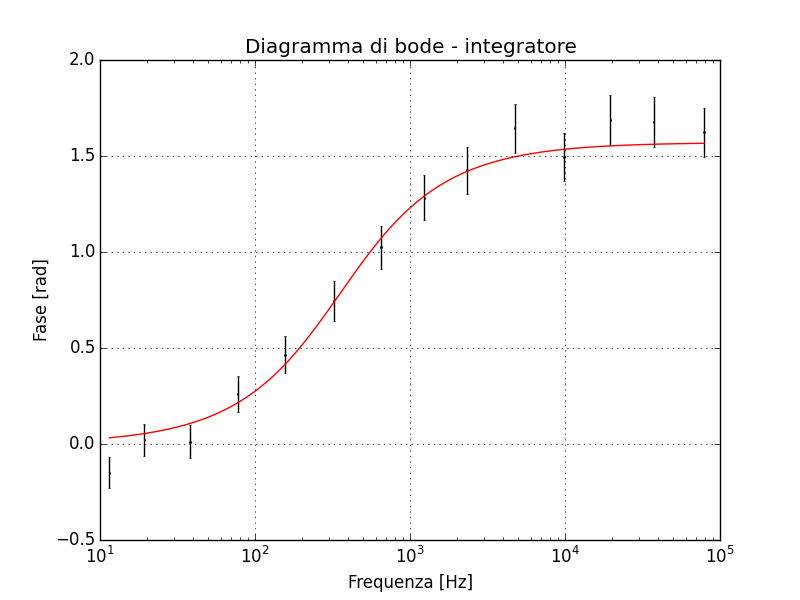
\includegraphics[width=0.8\textwidth]{../grafici/fit_phase_low_pass.pdf}
		\caption{Fase integratore}
		\label{fig:lowph}
	\end{figure}

Il modulo e la fase sono stati fittati con la funzione di trasferimento di un passabasso, con l'accortezza che la fase è traslata di $\pi$, poichè l'amplificatore è invertente. Si riportano nella tabella di seguito i risultati del fit:

\begin{table}[H]
\centering
\begin{tabular}{c|ccc}
amplitude	&	$A_0 = 9.71 \pm 0.22$	&	$f_0 = \unit{404 \pm 12}{\hertz}$	&	$\chi^2/ndof = 15.6 / 12$\\
phase		& &	$f_0 = \unit{350 \pm 40}{\hertz}$	&	$\chi^2/ndof = 10.7 / 13$
\end{tabular}
\end{table}

\noindent Dove si sono usati i seguenti simboli:
\begin{itemize}
\item $A_0$ è il guadagno di centro banda, in questo caso a basse frequenze;
%\item $\varphi_0$ è lo sfasamento per frequenze prossime allo 0;

\item $f_0$ è la frequenza di taglio dell'integratore.
\end{itemize}

Si nota dunque che le due misure della frequenza di taglio sono compatibili, a meno di $\sim 1\sigma$.

\subsection{Risposta all'onda quadra}

Qualitativamente il comportamento osservato per la risposta del circuito all'onda quadra è esattamente quello di un integratore, almeno a $\unit{10}{\kilo\hertz}$, come si osserva dalla \figurename{\ref{fig:intsq}}.

Cambiando la frequenza del segnale di input si osserva che per frequenze maggiori il segnale viene ulteriormente attenuato, ma qualitativamente preserva il funzionamento come integratore, mentre per frequenze più basse il condensatore ha il tempo di caricarsi del tutto e si può osservare una serie di esponenziali dovuti proprio a queste cariche e scariche, sempre in \figurename{\ref{fig:intsq}}.

\begin{figure}[H]
	\begin{minipage}[c]{0.49\textwidth}
		\centering
		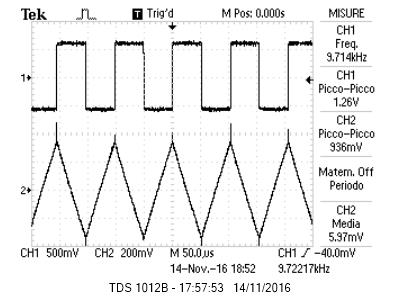
\includegraphics[width=1\textwidth]{../oscilloscopio/sqint.jpg}
	\end{minipage}
	\begin{minipage}[c]{0.49\textwidth}
		\centering
		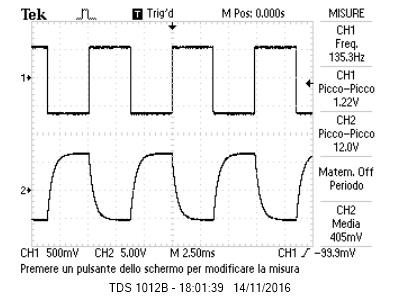
\includegraphics[width=1\textwidth]{../oscilloscopio/sqexp.jpg}
	\end{minipage}
	\caption{Risposta dell'integratore a un'onda quadra ($\sim\unit{10}{k\hertz}$ a sinistra e $\sim \unit{100}{\hertz}$ a destra)}
	\label{fig:intsq}
\end{figure}

Ci si aspetta che l'ampiezza dell'onda in uscita possa essere determinata da due fattori:
\begin{itemize}
\item lo slew rate finito;
\item l'integrazione dovuta al passa basso.
\end{itemize}

In questo caso, per frequenze dell'ordine della decina di kHz, lo slew rate finito non è rilevante, perché il segnale impiegherebbe meno di $\unit{1}{\micro\second}$ a raggiungere i  $\unit{10}{\volt}$, mentre il tempo di salita è il semiperiodo del segnale, quindi $\sim \unit{50}{\micro\second}$. Il comportamento è quindi dovuto alla pure integrazione, per cui il segnale sale con l'andamento $V_0(1 - e^{-t/\tau})$, che all'ordine più basso è un'andamento lineare $V_0 t/\tau$, con $\tau = R C = \unit{452 \pm 14}{\micro\second}$.

In approssimazione lineare il valore atteso per l'ampiezza è quindi $V_{out}^{exp} = \unit{900 \pm 40}{\milli\volt}$, che è compatibile con il valore misurato di $V_{out} = \unit{940 \pm 23}{\milli\volt}$.

%Il valore calcolato con l'esponenziale è invece $V_{out}^e = \unit{0.644 \pm 0.022}{\milli\volt}$, ma non torna quindi non ce lo scrivo

\subsection{Confronto con i risultati attesi}

Il valore della frequenza di taglio attesa dalla teoria è pari a $f_0^{exp} = \unit{352 \pm 11}{\hertz}$ ed è compatibile con quella misurata con il fit degli sfasamenti, e anche, a meno di $\sim 3\sigma$, con quanto ottenuto dal fit dei guadagni.

Come risulta dai grafici mostrati in \figurename{\ref{fig:lowamp}} e \figurename{\ref{fig:lowph}} il comportamento del circuito in esame è lo stesso di un passa-basso, con una funzione di trasferimento moltiplicata per un fattore $-R_2/R_1$, che quindi aumenta il guadagno massimo e inverte l'output, aggiungendo un $\pi$ alla fase di quest'ultimo.

La resistenza $R_2$ serve a spostare il polo dallo 0, e di conseguenza limitare il guadagno massimo del circuito, che altrimenti andrebbe a coincidere con quello dell'operazionale, un valore non stabilmente fissato. Invece in questo modo il massimo valore del guadagno è pari proprio a  $R_2/R_1$, come scritto sopra.
Idealmente è proprio per questo motivo che compare una frequenza di taglio: se l'amplificatore avesse un guadagno infinito il guadagno del circuito sarebbe una retta in assenza di $R_2$, per cui si comporterebbe da integratore a qualunque frequenza.

\section{Circuito derivatore}

Si è montato il circuito in \figurename{\ref{derivatore}}. I valori dei componenti usati nel montaggio del circuito coincidono con quelli al punto precedente.

\begin{figure}[H]
	\centering
	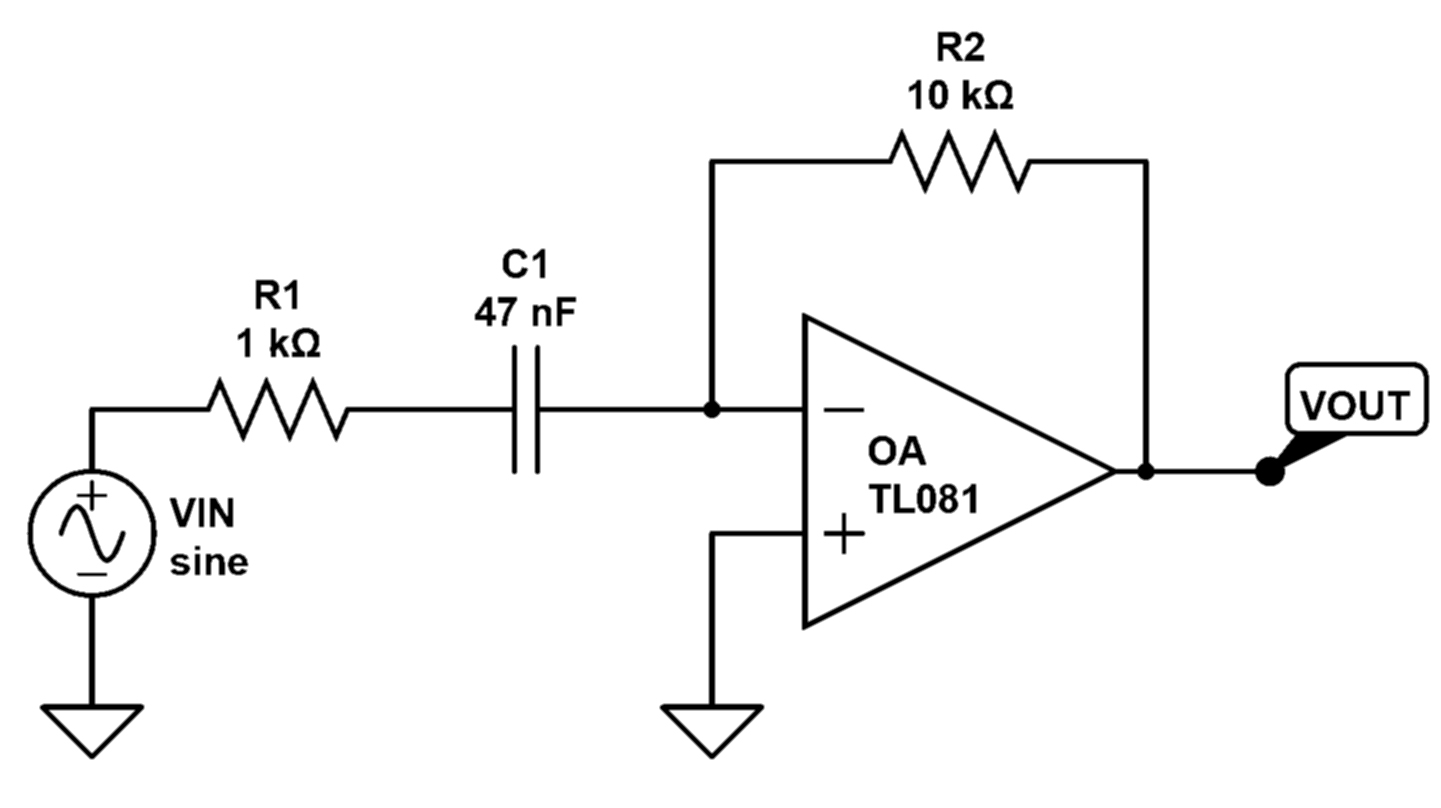
\includegraphics[width=0.4\textwidth]{../grafici/derivatore_circuito.jpg}
	\caption{Circuito derivatore}
	\label{derivatore}
\end{figure}

\subsection{Risposta in frequenza}

Come nel caso precedente si riportano i dati in appendice in \tablename{\ref{tab:highpass}} e i grafici di seguito, in \figurename{\ref{fig:highamp}} e \figurename{\ref{fig:highph}}.

	\begin{figure}[H]
		\centering
		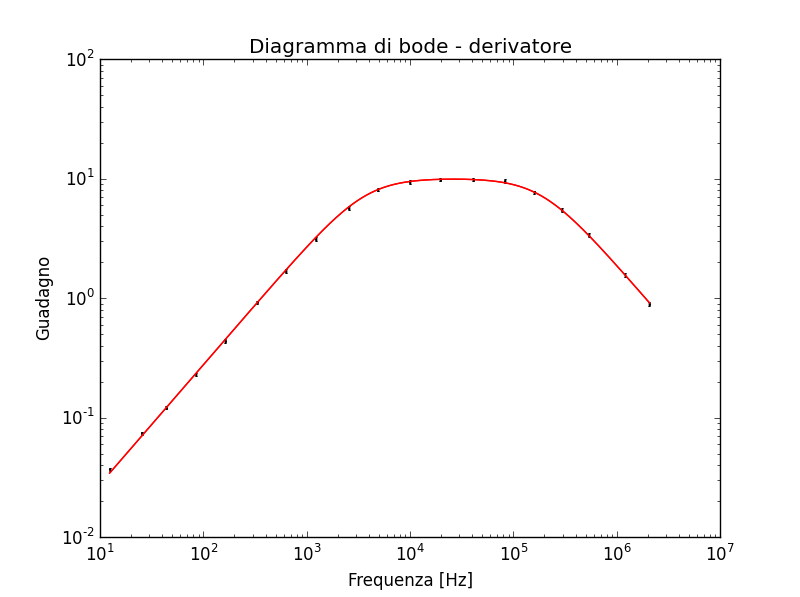
\includegraphics[width=0.8\textwidth]{../grafici/fit_module_high_pass.pdf}
		\caption{Guadagno derivatore}
		\label{fig:highamp}
	\end{figure}
	\begin{figure}[H]
		\centering
		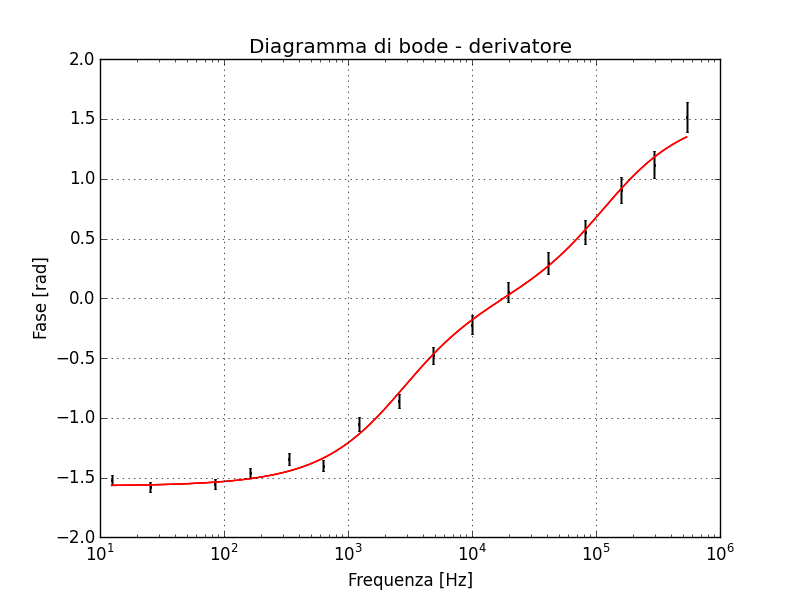
\includegraphics[width=0.76\textwidth]{../grafici/fit_phase_high_pass.pdf}
		\caption{Fase derivatore}
		\label{fig:highph}
	\end{figure}

Il modulo e la fase sono stati fittati con la funzione di trasferimento di un passa-banda, con l'accortezza che la fase è traslata di $\pi$, poiché l'amplificatore è invertente. Si riportano nella tabella di seguito i risultati del fit:

\begin{table}[H]
\centering
\begin{tabular}{c|cccc}
amplitude	&	$A_0 = 10.11 \pm 0.18$	&	$f_1 = \unit{3.64 \pm 0.08}{\kilo\hertz}$	&	$f_2 = \unit{189 \pm 6}{\kilo\hertz}$	&	$\chi^2/ndof = 8.6 / 16$\\
phase		& &	$f_1 = \unit{2.72 \pm 0.2}{\kilo\hertz}$	&	$f_2 = \unit{118 \pm 14}{\kilo\hertz}$	&	$\chi^2/ndof = 14.5 / 14$
\end{tabular}
\end{table}

\noindent Dove si è indicato con $f_1, f_2$ le due frequenze di taglio del circuito. La prima frequenza è relativa al derivatore, cioè quella fissata dal dimensionamento del circuito, mentre la seconda frequenza è quella relativa al taglio delle alte frequenze dovuto a effetti capacitivi imputabili all'op-amp. Come è chiaro le due stime di $f_1$ e $f_2$ non sono compatibili fra loro, dei due fit, quello che sembra dare risultati meno in linea con quanto atteso è il fit della fase per il quale tra l'altro sono stati trascurati gli ultimi due dati presi, che evidenziano chiaramente un andamento asintotico non in linea con il modello teorico.
\subsection{Risposta all'onda triangolare}
Alla frequenza di $\sim \unit{100}{\hertz}$ il circuito si comporta come un derivatore, come risulta dall'immagine riportata in \figurename{\ref{fig:trdev}}.

\begin{figure}[H]
\centering
	\begin{minipage}[c]{0.49\textwidth}
		\centering
		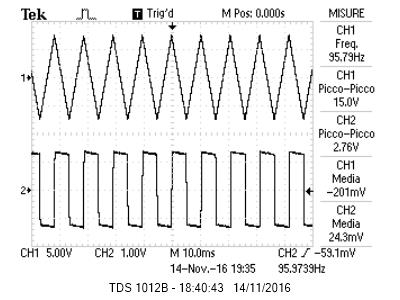
\includegraphics[width=0.85\textwidth]{../oscilloscopio/trdev.jpg}
		\caption{Risposta del circuito derivatore a un'onda triangolare in ingresso}
		\label{fig:trdev}
	\end{minipage}
	\begin{minipage}[c]{0.49\textwidth}
		\centering
		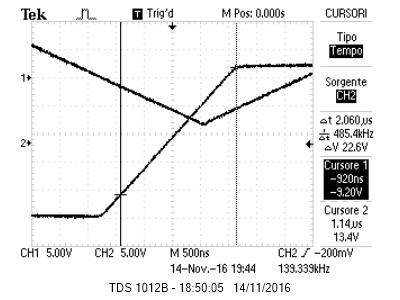
\includegraphics[width=0.85\textwidth]{../oscilloscopio/slewperf.jpg}
		\caption{Massima pendenza del segnale in uscita}
		\label{fig:slewperf}
	\end{minipage}
\end{figure}

Variando la frequenza si ha che per frequenze molto basse il condensatore si carica in un tempo breve rispetto alla durata del periodo, per cui la risposta approssima sempre meglio un'onda quadra e viene attenuata, come risulta dal grafico in \figurename{\ref{fig:highamp}}.

La massima pendenza osservata del segnale in uscita è mostrata in \figurename{\ref{fig:slewperf}}, e si ottiene che è pari a: $\unit{11.0 \pm 0.3}{\volt/\micro\second}$, cioè prossima allo \emph{slew rate}.

%perché non è esattamente quello son cazzi suoi... forse forse anche nostri...
%il gap sarà imputabile al derivatore

\subsection{Confronto con i risultati attesi}

Il valore atteso della frequenza di taglio dalla teoria è $f_1^{exp} = \unit{3.56 \pm 0.11}{\kilo\hertz}$, ed è perciò compatibile con quella ottenuta dal fit dei guadagni.

%rimane da giustificare perché le fasi non tornano

La funzione della resistenza $R_1$ è quella di aggiungere un polo, in modo tale da stabilizzare il circuito alle alte frequenze, cioé fissare il valore del massimo guadagno a un valore di progetto determinato dal dimensionamento delle resistenze e del condensatore.

Inoltre il circuito presenta un'altra frequenza di taglio, come si è notato ai punti precedenti. Questa non è prevista da un comportamento ideale del circuito in esame (in cui l'operazionale abbia una resistenza d'ingresso infinita e una di uscita nulla), ma tenendo di conto il comportamento reale dell'operazionale anche la seconda frequenza di taglio è spiegata. Il motivo è probabilmente il condensatore presente nell'operazionale, che secondo il datasheet ammonta a $\sim \unit{10}{\pico\farad}$.

Se si considera quest'ultimo condensatore come elemento di un passa basso si ottiene che per giustificare la frequenza di taglio trovata l'altro elemento dovrebbe essere una resistenza di $\sim \unit{100}{\kilo\ohm}$, che considerando il contributo dei transistor è plausibile, almeno come "resistenza efficace".

Anche in questo caso il guadagno massimo del circuito è moltiplicato per un valore $-R_2/R_1$, ma stavolta è ottenuto per alte frequenze, o meglio in una certa banda, prima che il segnale venga di nuovo attenuato.

\pagebreak
\section{Appendice: Dati acquisiti}
Si riportano qui le tabelle dei dati usati per i fit e i grafici.

\centering
\begin{figure}[h!]
	\begin{minipage}[t]{0.33\textwidth}
		\resizebox{1\textwidth}{!}{
		\input{../tabelle/tab_inv_amp_gain.txt}}
		\captionof{table}{Guadagno amplificatore invertente}
		\label{tab:inv_amp_gain}
	\end{minipage}
	\begin{minipage}[t]{0.33\textwidth}
		\resizebox{1\textwidth}{!}{
		\input{../tabelle/tab_inv_amp_f_domain.txt}}
		\captionof{table}{Risposta in frequenza amplificatore invertente}
		\label{tab:inv_amp_f_domain}
	\end{minipage}
	\begin{minipage}[t]{0.33\textwidth}
		\resizebox{1\textwidth}{!}{
			\input{../tabelle/tab_gain_bandwidth.txt}}
		\captionof{table}{Banda/Guadagno}
		\label{tab:gain_bandwidth}
	\end{minipage}
\end{figure}

\begin{figure}[h!]
	\centering
	\resizebox{0.7\textwidth}{!}{
	\input{../tabelle/tab_low_pass.txt}}
	\captionof{table}{Dati relativi al circuito integratore}
	\label{tab:lowpass}
\end{figure}

\begin{figure}[H]
	\centering
	\resizebox{0.7\textwidth}{!}{
	\input{../tabelle/tab_high_pass.txt}}
	\captionof{table}{Dati relativi al circuito derivatore}
	\label{tab:highpass}
\end{figure}



\end{document}
